% !TeX root = ../thuthesis-example.tex

\chapter{应用:封装稀疏矩阵分解算法}

\section{背景介绍}

Cholesky 分解是一种重要的矩阵分解方式,常被应用在对称线性系统求解问题中。很多实际问题中,矩阵的规模过大,为了对其进行 Cholesky 分解,需要专门针对稀疏矩阵数据结构的分解算法。

SciPy 和 NumPy\cite{harris2020array} 是著名的 Python 科学计算库,遗憾的是,它们并没有提供稀疏矩阵 Cholesky 分解功能;而另一方面,以 C 语言实现的 SuiteSparse 库高效地实现了稀疏矩阵 Cholesky 分解算法,集成在其子模块 CHOLMOD 中。本章基于 CPP2PY 封装 CHOLMOD,使其能接受 SciPy 稀疏矩阵输入,从而使其 具备了大规模稀疏矩阵的高效 Cholesky 分解功能。与直接使用C语言编程相比,性能损失在 5\% 以下。

\section{理论知识}

本节简明扼要地介绍了稀疏 Cholesky 分解理论\cite{sparsesurvey, 邹丹2014基于,喻文健2015数值分析与算法} 。我们略去细节证明,聚焦于算法流程和基本思想。尽管这些内容与跨语言接口开发没有直接关系,了解它们有助于理清 CHOLMOD 库的工作方式。

\subsection{稀疏矩阵数据结构}

稀疏矩阵中非零元素占比很小,为了节省空间,常采用压缩存储数据结构,常见的存储格式包括三元组(COO)、压缩稀疏行(CSR)、压缩稀疏列(CSC)等。各种稀疏矩阵算法就是专门针对稀疏矩阵特殊的存储格式设计的。

CHOLMOD 库的稀疏矩阵基于压缩稀疏列结构,此种数据结构结构将非零元按列顺序存储,不需要记录每个元素的列号,只需记录每列第一个非零元的位置。一个压缩稀疏列矩阵包含三个数组:非零元素值(val)、行编号数组(row)、列指针数据(pcol)。下面是一个 CSC 格式的稀疏矩阵的例子。

\begin{equation}
A = \begin{bmatrix}
1 & 0 & 2 & 0 & 0\\
3 & 4 & 0 & 5 & 0\\
6 & 0 & 7 & 0 & 8\\
0 & 9 & 0 & 6 & 0\\
0 & 0 & 0 & 0 & 7
\end{bmatrix}    
\end{equation}

\begin{figure}
  \centering
  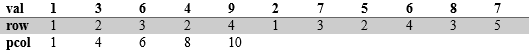
\includegraphics[width=0.8\linewidth]{figures/稀疏矩阵.png}
  \caption{矩阵 A 的 CSC 格式存储}
  \label{fig:4.1}
\end{figure}

\subsection{消去树}

稀疏 Cholesky 分解算法分为符号分析和数值分解两个阶段。在符号分析阶段,算法分析矩阵的非零模式,为后继的数值分解阶段做准备,使数值求解的时空复杂度都大幅下降;数值分解阶段将计算出分解的结果。与数值分解相比,符号分析的开销相对较小。

在整个算法中,消去树(elimination tree)是一个绕不开的概念,它指导了Cholesky分解的符号分析阶段,也为数值分解提供了一个基本框架。

形式上,$n$ 阶对称正定矩阵 $A=(a_{ij})$ 诱导出一个包含 $n$ 个节点的图 $G_A=(V_A, E_A)$,其中 $V_A=\{0,⋯,n-1\},E_A=\{(i,j)|0≤ j<i<n,  a_{ij}≠0\}$ 。

对于 Cholesky 分解 $A=LL^T, A=(a_{ij}), L=(l_{ij})$,有如下两个命题成立:

\begin{theorem}\label{theorem:1} 如果 $ a_{ij}\ne0 $,则 $l_{ij}\ne 0$。\end{theorem}
\begin{theorem}\label{theorem:2} 如果 $i<j<k$ 且  $l_{ji}\ne 0$,$l_{ki}\ne 0$,则 $l_{kj}\ne 0$ 。\end{theorem}

从定理 \ref{theorem:1} 可以知道,$L$ 继承了 $A$ 的所有非零模式。定理 \ref{theorem:2} 告诉我们,若在图 $G_L$ 中有 $(i, j)\in E_L$,则对所有 $k>j$ ,边 $(i, k)$ 实际上是冗余的,因为从节点 $i$ 可以途经 $j$ 到达 $k$。

由此可以对 $G_L$ 做剪枝,每个节点 $i$ 只需要维护至多一条出边 $(i,parent(i))$,其中 $parent(i)=\min(j:(i,j)\in E_L)$ ,这样得到的图称为矩阵 $A$ 的消去树。

\begin{figure}
  \centering
  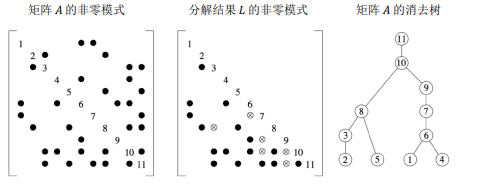
\includegraphics[width=0.8\linewidth]{figures/消去树.png}
  \caption{某矩阵的 Cholesky 分解和消去树}
  \label{fig:4.2}
\end{figure}

\subsection{符号分析}

在 Cholesky 分解过程中,矩阵 $L$ 在继承 $A$ 的所有非零模式基础上会增加一些新的非零元,称为填入元(fill-in)。图 \ref{fig:4.2} 中分解结果 $L$ 中的空心圈就是填入元。填入元会造成分解结果的稀疏性下降,进而提高算法的空间和时间复杂度。

在符号分解阶段,首先会寻找一个排列阵 $P$,称为减少填入排列,使得 $PAP^T$ 的分解结果中填入元尽量少。求最优减少填入排列是一个 NP 难问题,实践中一般采用启发式算法。

减少填入排列确定后,符号分析将对 $A$ 进行符号分解,计算出 $L$ 的非零模式,以消去树的形式给出。

\subsection{数值分解}

CHOLMOD 提供了两种数值求解方法,分别基于向上查看法和向左查看法。

向上查看法在每轮迭代中计算出矩阵 $L$ 的一行,因此也被称为行 Cholesky 算法。考虑等式 $A=LL^T$ 的如下分块:
\begin{equation}
\begin{bmatrix}
L_{11} & \\
l_{12}^T & l_{22}
\end{bmatrix}
\begin{bmatrix}
L_{11}^T & l_{12}\\
 & l_{22}
\end{bmatrix}=
\begin{bmatrix}
A_{11} & a_{12}\\
a_{12}^T & a_{22}
\end{bmatrix}
\end{equation}
其中 $l_{12}, a_{12}$ 为 $n-1$ 维向量; $l_{22}, a_{22}$ 为标量;$A_{11}$ 是原矩阵左上角的 $n-1$ 阶子矩阵,其 Cholesky 分解为 $L_{11}$。假设我们已经求出了前 $n-1$ 行的分解结果,即矩阵 $L_{11}$,则由分块矩阵乘法可得,
\begin{align}
l_{12}&=L_{11}/ a_{12}\\
a_{22}&=l_{12}^T l_{12}+l_{22}^2
\end{align}其中 “/” 符号表示求解三角方程组。

向上查看法的伪代码如算法 \ref{alg1} 所示,它在经过一些特别的优化后可用于稀疏矩阵的分解,当矩阵特别稀疏时,该方法比很多复杂方法更有效。

\begin{algorithm}
  \caption{向上查看Cholesky分解}
  \label{alg1}
  \small
  \begin{algorithmic}
  \REQUIRE 矩阵 $A$
  \ENSURE Cholesky 因子 $L$
  \FOR{k = 1 \TO n}
  \STATE $L_{k,1:k-1} \gets L_{1:k-1,1:k-1}/A_{1:k-1,k}$
  \STATE $L_{k,k} \gets \sqrt{A_{k,k} \minus L_{k,1:k-1} L_{k:1:k-1}^T} $  
  \ENDFOR
  \end{algorithmic}
\end{algorithm}

向左查看 Cholesky 分解算法在每轮迭代中计算出矩阵 $L$ 的一列,因此也被称为列 Cholesky 算法。在迭代进行至第 $k$ 轮时,考虑等式 $A=LL^T$ 的如下分块:
\begin{equation}
\begin{bmatrix}
L_{11} & &\\
l_{12}^T & l_{22} & \\
L_{31} & l_{32} & L_{33}
\end{bmatrix}
\begin{bmatrix}
L_{11}^T & l_{12} & L^T_{31}\\
 & l_{22} & l_{32}^T \\
 &  & L_{33}^T
\end{bmatrix}
=  \begin{bmatrix}
A_{11} & a_{12} & A_{31}^T\\
a_{12}^T & a_{22} &  a_{32}^T\\
A_{31} & a_{32} & A_{33}
\end{bmatrix}
\end{equation}
其中 $[L_{11};l_{12}^T;L_{31}]$ 是已经求出的前 $k-1$ 列,$[l_{22};l_{32}]$ 为待求列,$l_{22}$ 为标量。引入一个 $n-k+1$ 维的向量 $c$,根据分块矩阵乘法,可得待求列与已求列之间的关系:
\begin{align}
c &= \begin{bmatrix}
c_1 \\
c_2
\end{bmatrix} = 
\begin{bmatrix}
a_{22} \\
a_{32}
\end{bmatrix} - \begin{bmatrix}
l_{12}^T \\
L_{31}
\end{bmatrix}l_{12} \\
l_{22}&=\sqrt{c_1}\\
l_{32}&=c_2/l_{22}
\end{align}

根据这一递推关系,可以得到向左查看算法。这种算法能针对稀疏矩阵做多种优化。注意到,计算向量 $c$ 时,只需要考虑 $A$ 中的非零列,当我们分析出 $A$ 的非零元模式后,向量 $c$ 的计算效率将大大增加。向左查看法借助消去树的指导,可以分为很多子任务,更适合并行计算。向左查看法很容易改造为分块的版本,这构成了超节点(Supernodal)Cholesky 分解的基础。

\begin{algorithm}
  \caption{向左查看Cholesky分解}
  \label{alg2}
  \small
  \begin{algorithmic}
  \REQUIRE 矩阵 $A$
  \ENSURE Cholesky 因子 $L$
  \FOR{k = 1 \TO n}
  \STATE $c_{k:n}=A_{k:n,k}-L_{k:n,1:k-1} L_{k,1:k-1}^T$
  \STATE $L_{k,k}=\sqrt{c_k}$
  \STATE $L_{k+1:n,k}=c_{k+1:n,k}/L_{k,k}$
  \ENDFOR
  \end{algorithmic}
\end{algorithm}

\section{程序实现}

程序实现主要分为两步,调用 CPP2PY 自动生成代码,并在此基础上进行二次开发。

CHOLMOD\cite{chen2008algorithm, davis2008user} 库完成 Cholesky 分解需要调用的例程主要有两个:\lstinline{cholmod_analyze} 和 \lstinline{cholmod_factorize},前者进行符号分析,后者完成数值分解。调用 \lstinline{cholmod_analyze} 时需要给出寻找减小填入排列和数值分解的方法。

CHOLMOD 主要提供了两种计算减填序列的方法,近似最小度数法(Approximate Minimum Degree)和嵌套分割方法(Nested dissection),METIS 是后者的一个实现。受支持的数值分解方法有两种:simplicial(基于向上查看法)和 supernodal(基于向左查看的超节点法)。\lstinline{cholmod_analyze} 根据选择的数值分解算法返回不同的符号分析结果。

减少填入排列和分解方法都选定后,\lstinline{cholmod_analyze} 例程被调用,返回一个 \lstinline{cholmod_factor} 结构体,该结构作为 \lstinline{cholmod_factorize} 的输入,指导后者进行数值分解。

CPP2PY 能正确地解析 CHOLMOD 库的源程序,但考虑到算法库体量庞大,包含了上百个 API 接口,其中与 Cholesky 分解直接相关的只有十多个,直接解析源程序将生成大量无关代码。为了后续开发的方便,可以将源程序头文件中有用的部分手动提取出来,让 CPP2PY 只解析这部分子集。为了处理泛型指针 \lstinline{void*} ,需要编写类型转换器子类,根据属性名指定泛型指针的实际类型。

\begin{algorithm}
  \caption{将 \lstinline$scipy.sparse$ 稀疏矩阵转换为 \lstinline$cholmod_sparse$}
  \label{alg3}
  \small
  \begin{algorithmic}
  \REQUIRE \lstinline$scipy.sparse$ 矩阵 $m$
  \ENSURE \lstinline$cholmod_sparse$ 矩阵 $out$
  \IF{not m.iscsc()}
    \STATE m = m.tocsc()
  \ENDIF
  \STATE 根据 $m$ 中的数据,初始化 $out$
  \RETURN $out$
  \end{algorithmic}
\end{algorithm}


\begin{algorithm}
  \caption{将 \lstinline$cholmod_sparse$ 稀疏矩阵转换为 \lstinline$scipy.sparse$}
  \label{alg4}
  \small
  \begin{algorithmic}
  \REQUIRE \lstinline$cholmod_sparse$ 矩阵 $m$
  \ENSURE \lstinline$scipy.sparse$ 矩阵 $out$
  \STATE 根据 $m$ 中的数据,调用 NumPy C API,初始化 $out$ 对象
  \STATE 为 $out$ 重写析构函数,保证 $out$ 被析构时内存被正确释放
  \RETURN $out$
  \end{algorithmic}
\end{algorithm}

CHOLMOD 根据不同的数据结构和上下文提供了分配、回收内存的多个例程,CPP2PY 不知道该如何调用这些例程。二次开发中需要手动处理内存释放问题。

类型转换是跨语言接口的关键部分。\lstinline{scipy.sparse} 模块定义了多种稀疏矩阵类,而 CHOLMOD 使用的稀疏矩阵 \lstinline{cholmod_sparse} 以 CSC 格式存储。为了让封装后的CHOLMOD能分解 \lstinline{scipy.sparse} 稀疏矩阵,要实现后者与 \lstinline{cholmod_sparse} 之间的相互转换。伪代码如算法 \ref{alg3} 和 \ref{alg4} 所示,实现中尽可能避免了大块数据的复制和移动,从而保证了类型转换的效率。

封装后的Cholesky分解算法伪代码如算法 \ref{alg5} 所示。

\begin{algorithm}
  \caption{稀疏Cholesky分解Python接口}
  \label{alg5}
  \small
  \begin{algorithmic}
  \REQUIRE \lstinline$scipy.sparse$ 矩阵 $A$,分解模式 mode,排序方法 ordering\_method
  \ENSURE \lstinline$scipy.sparse$ 格式的 Cholesky 因子 $L$
  \STATE 将 $A$ 转换为 \lstinline$cholmod_sparse$ 稀疏矩阵 $m$
  \STATE 初始化参数
  \STATE 调用 \lstinline$cholmod_analyze$ 进行符号分析,得到 $factor$
  \STATE 调用 \lstinline$cholmod_factorize$ 分解 $factor$
  \STATE 将 $factor$ 转换为 \lstinline$scipy.sparse$ 稀疏矩阵 $L$
  \RETURN $L$
  \end{algorithmic}
\end{algorithm}

\section{实验测试}

\subsection{实验设置}

实验的系统环境 Ubuntu 20.04,CPU 为 AMD(R) RYZEN(TM) 5800H,SuiteSparse 版本为 5.7.1,CHOLMOD 版本为 3.0.14,Python 和 SciPy 的版本分别为 3.8.10 和 1.6.3。实验以直接用 C 语言调用 CHOLMOD 为基线,验证调用 Python 接口分解稀疏矩阵的结果是否与之一致,并比较二者的性能。

为了规避 OS 调度等因素的影响,性能测试的标准为多次运行取最优。Cholesky 分解策略指定为以下四种:Simplicial/AMD、Simplicial/METIS、Supernodal/AMD、Supernodal/METIS。这些策略的详细含义见上一节。

\begin{table}
  \centering
  \caption{测例矩阵}
  \begin{tabular}{lll}
    \toprule
     测例           &  行/列数  &  下三角非零元数 \\
    \midrule
     ted\_B          &  10605    &  77592          \\
     s3rmt3m3       &  5357     &  106526         \\
     thermomech\_dM  &  204316   &  813716         \\
     parabolic\_fem  &  525825   &  2100225        \\
     nd12k          &  36000    &  7128473        \\
     nd24k          &  72000    &  14393817       \\
     PFlow\_742      &  742793   &  18940627       \\
     boneS10        &  914898   &  28191660       \\
    \bottomrule
  \end{tabular}
  \label{tab:4.1}
\end{table}


实验测试数据\footnote{数据来源于 \url{https://sparse.tamu.edu/}.}罗列如表 \ref{tab:4.1},它们均为对称正定矩阵。这些矩阵规模庞大,只能以稀疏形式存储。图 \ref{fig:4.3} 展示了它们的非零元模式。


\begin{figure}
  \centering
  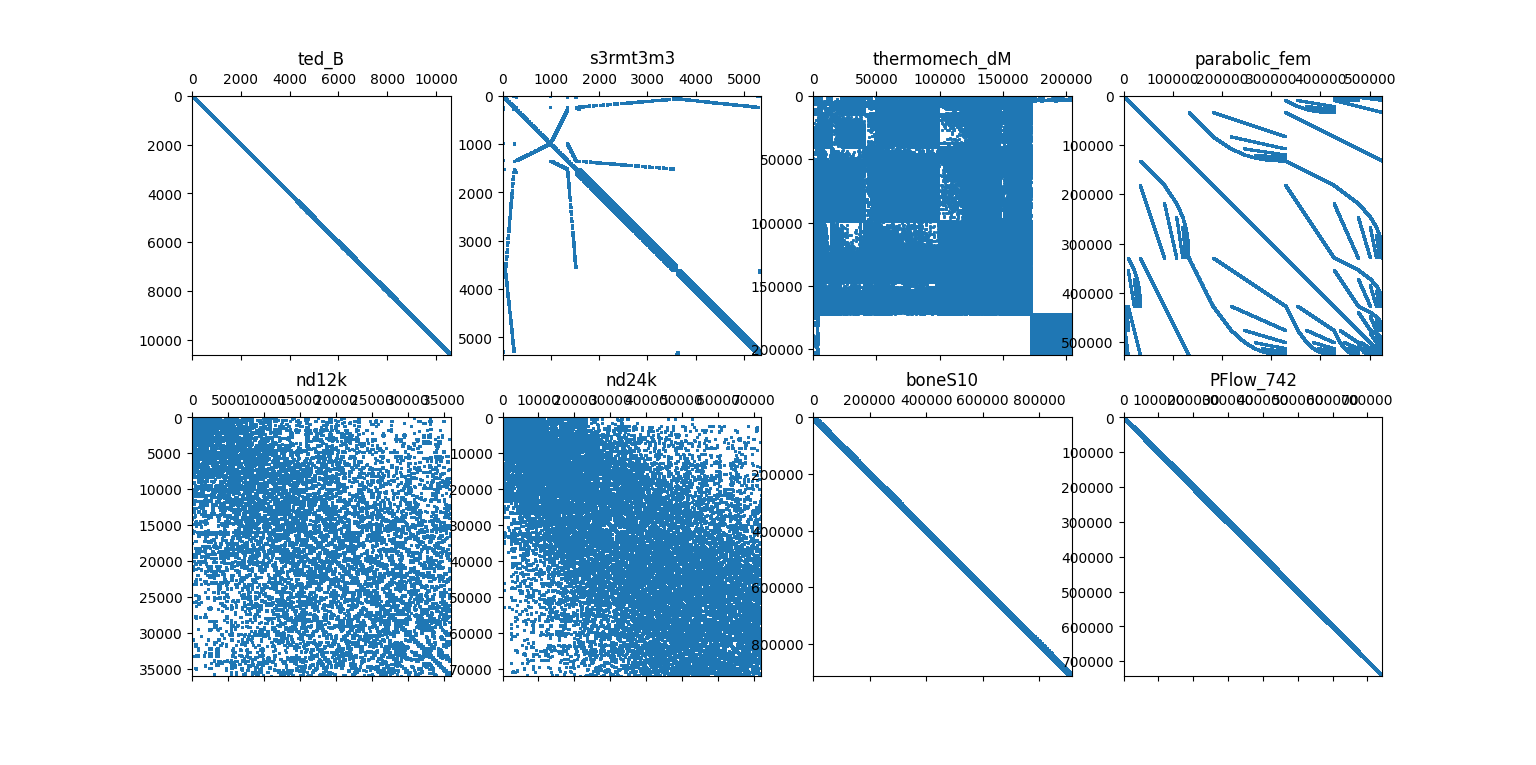
\includegraphics[width=\linewidth]{figures/测例矩阵.png}
  \caption{测例矩阵的非零元模式}
  \label{fig:4.3}
\end{figure}

\subsection{实验结果}

调用 Python 接口的分解结果与直接编写 C 程序得到的结果在误差范围内一致,确保了实验的正确性。

由表 \ref{tab:4.21} 可知,与直接以 C 语言编程相比,调用 Python 接口进行分解花费的额外时间占原耗时比例通常在 5\% 以内。性能测试的原始数据见附录表 \ref{tab:4.2} 和 \ref{tab:4.3}。

\begin{table}
  \centering
  \caption{Python 接口相对 C 的额外开销占原耗时比例}
  \begin{tabular}{lllll}
    \toprule
     测例           &  Simplicial/AMD  &  Simplicial/METIS  &  Supernodal/AMD  &  Supernodal/METIS \\
    \midrule
    ted\_B & 2.01\% & 4.35\% & 2.24\% & 8.47\% \\
 s3rmt3m3       &        0.50\% & 4.39\% & 4.88\% & 6.04\% \\
thermomech\_dM  &        0.33\% & 0.02\% & 0.25\% & 5.31\% \\
parabolic\_fem  &        0.09\% & 0.99\% & 1.83\% & 1.36\% \\
nd12k          &         0.06\% & 0.26\% & 0.66\% & 0.16\% \\
nd24k          &       0.14\% & 0.50\% & 0.09\% & 0.09\% \\
PFlow\_742      &        0.01\% & 0.05\% & 0.23\% & 0.32\% \\
boneS10        &        0.11\% & 0.24\% & 0.31\% & 0.66\% \\
    \bottomrule
  \end{tabular}
  \label{tab:4.21}
\end{table}
